% Created by tikzDevice version 0.10.1 on 2016-07-18 19:10:44
% !TEX encoding = UTF-8 Unicode
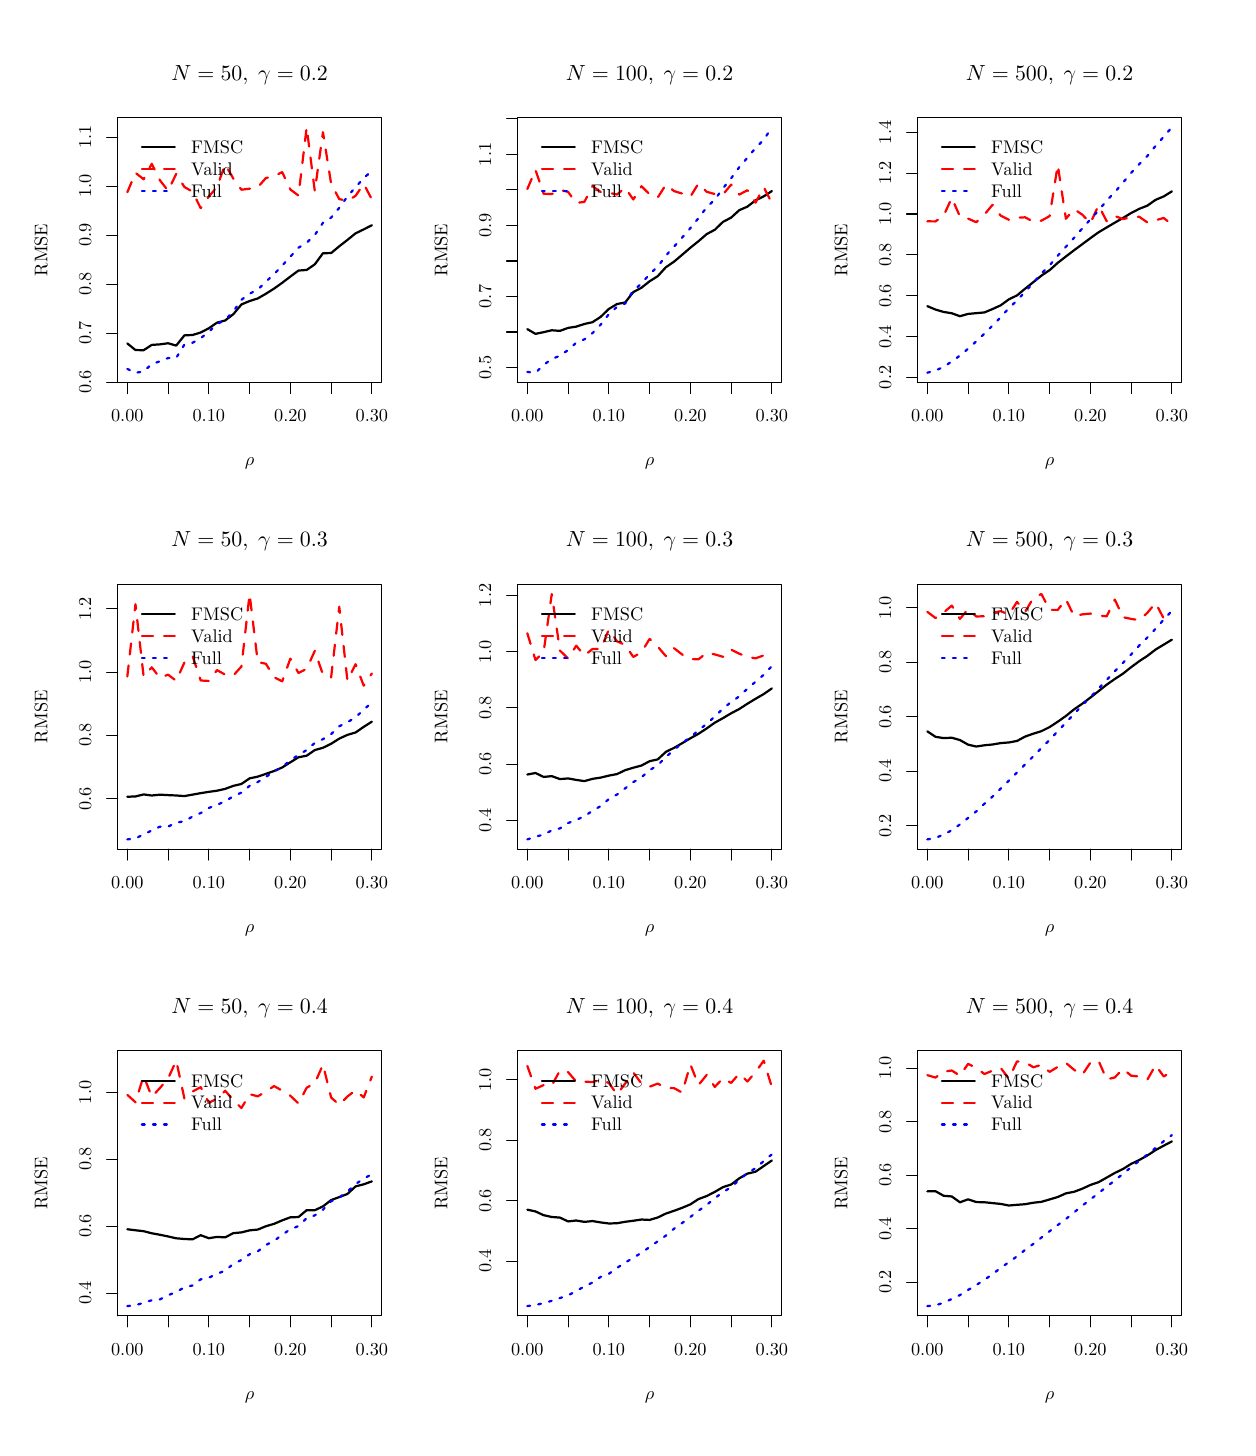
\begin{tikzpicture}[x=1pt,y=1pt]
\definecolor{fillColor}{RGB}{255,255,255}
\path[use as bounding box,fill=fillColor,fill opacity=0.00] (0,0) rectangle (433.62,505.89);
\begin{scope}
\path[clip] ( 32.47,377.65) rectangle (127.91,473.42);
\definecolor{drawColor}{RGB}{0,0,0}

\path[draw=drawColor,line width= 0.8pt,line join=round,line cap=round] ( 36.01,391.78) --
	( 38.95,389.39) --
	( 41.90,389.33) --
	( 44.84,391.25) --
	( 47.79,391.45) --
	( 50.73,391.85) --
	( 53.68,391.00) --
	( 56.63,394.70) --
	( 59.57,394.83) --
	( 62.52,395.73) --
	( 65.46,397.26) --
	( 68.41,399.29) --
	( 71.35,400.08) --
	( 74.30,402.33) --
	( 77.24,405.87) --
	( 80.19,407.10) --
	( 83.14,408.04) --
	( 86.08,409.73) --
	( 89.03,411.60) --
	( 91.97,413.69) --
	( 94.92,415.95) --
	( 97.86,418.12) --
	(100.81,418.34) --
	(103.75,420.36) --
	(106.70,424.37) --
	(109.65,424.44) --
	(112.59,426.89) --
	(115.54,429.18) --
	(118.48,431.57) --
	(121.43,432.99) --
	(124.37,434.49);
\end{scope}
\begin{scope}
\path[clip] (  0.00,  0.00) rectangle (433.62,505.89);
\definecolor{drawColor}{RGB}{0,0,0}

\path[draw=drawColor,line width= 0.4pt,line join=round,line cap=round] ( 36.01,377.65) -- (124.37,377.65);

\path[draw=drawColor,line width= 0.4pt,line join=round,line cap=round] ( 36.01,377.65) -- ( 36.01,373.69);

\path[draw=drawColor,line width= 0.4pt,line join=round,line cap=round] ( 50.73,377.65) -- ( 50.73,373.69);

\path[draw=drawColor,line width= 0.4pt,line join=round,line cap=round] ( 65.46,377.65) -- ( 65.46,373.69);

\path[draw=drawColor,line width= 0.4pt,line join=round,line cap=round] ( 80.19,377.65) -- ( 80.19,373.69);

\path[draw=drawColor,line width= 0.4pt,line join=round,line cap=round] ( 94.92,377.65) -- ( 94.92,373.69);

\path[draw=drawColor,line width= 0.4pt,line join=round,line cap=round] (109.65,377.65) -- (109.65,373.69);

\path[draw=drawColor,line width= 0.4pt,line join=round,line cap=round] (124.37,377.65) -- (124.37,373.69);

\node[text=drawColor,anchor=base,inner sep=0pt, outer sep=0pt, scale=  0.66] at ( 36.01,363.40) {0.00};

\node[text=drawColor,anchor=base,inner sep=0pt, outer sep=0pt, scale=  0.66] at ( 65.46,363.40) {0.10};

\node[text=drawColor,anchor=base,inner sep=0pt, outer sep=0pt, scale=  0.66] at ( 94.92,363.40) {0.20};

\node[text=drawColor,anchor=base,inner sep=0pt, outer sep=0pt, scale=  0.66] at (124.37,363.40) {0.30};

\path[draw=drawColor,line width= 0.4pt,line join=round,line cap=round] ( 32.47,377.78) -- ( 32.47,466.35);

\path[draw=drawColor,line width= 0.4pt,line join=round,line cap=round] ( 32.47,377.78) -- ( 28.51,377.78);

\path[draw=drawColor,line width= 0.4pt,line join=round,line cap=round] ( 32.47,395.49) -- ( 28.51,395.49);

\path[draw=drawColor,line width= 0.4pt,line join=round,line cap=round] ( 32.47,413.21) -- ( 28.51,413.21);

\path[draw=drawColor,line width= 0.4pt,line join=round,line cap=round] ( 32.47,430.92) -- ( 28.51,430.92);

\path[draw=drawColor,line width= 0.4pt,line join=round,line cap=round] ( 32.47,448.63) -- ( 28.51,448.63);

\path[draw=drawColor,line width= 0.4pt,line join=round,line cap=round] ( 32.47,466.35) -- ( 28.51,466.35);

\node[text=drawColor,rotate= 90.00,anchor=base,inner sep=0pt, outer sep=0pt, scale=  0.66] at ( 22.97,377.78) {0.6};

\node[text=drawColor,rotate= 90.00,anchor=base,inner sep=0pt, outer sep=0pt, scale=  0.66] at ( 22.97,395.49) {0.7};

\node[text=drawColor,rotate= 90.00,anchor=base,inner sep=0pt, outer sep=0pt, scale=  0.66] at ( 22.97,413.21) {0.8};

\node[text=drawColor,rotate= 90.00,anchor=base,inner sep=0pt, outer sep=0pt, scale=  0.66] at ( 22.97,430.92) {0.9};

\node[text=drawColor,rotate= 90.00,anchor=base,inner sep=0pt, outer sep=0pt, scale=  0.66] at ( 22.97,448.63) {1.0};

\node[text=drawColor,rotate= 90.00,anchor=base,inner sep=0pt, outer sep=0pt, scale=  0.66] at ( 22.97,466.35) {1.1};

\path[draw=drawColor,line width= 0.4pt,line join=round,line cap=round] ( 32.47,377.65) --
	(127.91,377.65) --
	(127.91,473.42) --
	( 32.47,473.42) --
	( 32.47,377.65);
\end{scope}
\begin{scope}
\path[clip] (  0.00,337.26) rectangle (144.54,505.89);
\definecolor{drawColor}{RGB}{0,0,0}

\node[text=drawColor,anchor=base,inner sep=0pt, outer sep=0pt, scale=  0.79] at ( 80.19,486.92) {\bfseries $N=50, \;\gamma=0.2$};

\node[text=drawColor,anchor=base,inner sep=0pt, outer sep=0pt, scale=  0.66] at ( 80.19,347.56) {$\rho$};

\node[text=drawColor,rotate= 90.00,anchor=base,inner sep=0pt, outer sep=0pt, scale=  0.66] at (  7.13,425.53) {RMSE};
\end{scope}
\begin{scope}
\path[clip] ( 32.47,377.65) rectangle (127.91,473.42);
\definecolor{drawColor}{RGB}{255,0,0}

\path[draw=drawColor,line width= 0.8pt,dash pattern=on 4pt off 4pt ,line join=round,line cap=round] ( 36.01,446.41) --
	( 38.95,453.44) --
	( 41.90,451.11) --
	( 44.84,456.70) --
	( 47.79,450.74) --
	( 50.73,446.94) --
	( 53.68,453.05) --
	( 56.63,448.32) --
	( 59.57,446.61) --
	( 62.52,440.66) --
	( 65.46,444.87) --
	( 68.41,448.31) --
	( 71.35,456.51) --
	( 74.30,451.38) --
	( 77.24,447.33) --
	( 80.19,447.71) --
	( 83.14,448.22) --
	( 86.08,451.55) --
	( 89.03,452.25) --
	( 91.97,453.68) --
	( 94.92,447.42) --
	( 97.86,445.20) --
	(100.81,469.87) --
	(103.75,446.86) --
	(106.70,468.12) --
	(109.65,449.48) --
	(112.59,443.95) --
	(115.54,443.29) --
	(118.48,445.13) --
	(121.43,449.41) --
	(124.37,443.86);
\definecolor{drawColor}{RGB}{0,0,255}

\path[draw=drawColor,line width= 0.8pt,dash pattern=on 1pt off 3pt ,line join=round,line cap=round] ( 36.01,382.57) --
	( 38.95,381.20) --
	( 41.90,381.63) --
	( 44.84,384.36) --
	( 47.79,385.33) --
	( 50.73,386.49) --
	( 53.68,386.56) --
	( 56.63,391.37) --
	( 59.57,392.03) --
	( 62.52,393.66) --
	( 65.46,396.02) --
	( 68.41,398.72) --
	( 71.35,400.32) --
	( 74.30,403.32) --
	( 77.24,407.55) --
	( 80.19,409.75) --
	( 83.14,411.23) --
	( 86.08,414.08) --
	( 89.03,416.81) --
	( 91.97,419.90) --
	( 94.92,423.13) --
	( 97.86,426.38) --
	(100.81,428.17) --
	(103.75,430.96) --
	(106.70,435.37) --
	(109.65,437.26) --
	(112.59,440.77) --
	(115.54,444.87) --
	(118.48,448.24) --
	(121.43,451.53) --
	(124.37,454.16);
\definecolor{drawColor}{RGB}{0,0,0}

\path[draw=drawColor,line width= 0.8pt,line join=round,line cap=round] ( 41.28,462.63) -- ( 53.16,462.63);
\definecolor{drawColor}{RGB}{255,0,0}

\path[draw=drawColor,line width= 0.8pt,dash pattern=on 4pt off 4pt ,line join=round,line cap=round] ( 41.28,454.71) -- ( 53.16,454.71);
\definecolor{drawColor}{RGB}{0,0,255}

\path[draw=drawColor,line width= 0.8pt,dash pattern=on 1pt off 3pt ,line join=round,line cap=round] ( 41.28,446.79) -- ( 53.16,446.79);
\definecolor{drawColor}{RGB}{0,0,0}

\node[text=drawColor,anchor=base west,inner sep=0pt, outer sep=0pt, scale=  0.66] at ( 59.10,460.35) {FMSC};

\node[text=drawColor,anchor=base west,inner sep=0pt, outer sep=0pt, scale=  0.66] at ( 59.10,452.43) {Valid};

\node[text=drawColor,anchor=base west,inner sep=0pt, outer sep=0pt, scale=  0.66] at ( 59.10,444.51) {Full};
\end{scope}
\begin{scope}
\path[clip] (177.01,377.65) rectangle (272.45,473.42);
\definecolor{drawColor}{RGB}{0,0,0}

\path[draw=drawColor,line width= 0.8pt,line join=round,line cap=round] (180.55,396.95) --
	(183.49,395.25) --
	(186.44,395.86) --
	(189.38,396.54) --
	(192.33,396.32) --
	(195.27,397.40) --
	(198.22,397.85) --
	(201.17,398.82) --
	(204.11,399.46) --
	(207.06,401.40) --
	(210.00,404.24) --
	(212.95,406.02) --
	(215.89,406.58) --
	(218.84,410.34) --
	(221.78,411.91) --
	(224.73,414.24) --
	(227.68,416.10) --
	(230.62,419.33) --
	(233.57,421.34) --
	(236.51,423.83) --
	(239.46,426.37) --
	(242.40,428.72) --
	(245.35,431.28) --
	(248.29,432.86) --
	(251.24,435.70) --
	(254.19,437.25) --
	(257.13,439.93) --
	(260.08,441.22) --
	(263.02,443.50) --
	(265.97,444.94) --
	(268.91,446.84);
\end{scope}
\begin{scope}
\path[clip] (  0.00,  0.00) rectangle (433.62,505.89);
\definecolor{drawColor}{RGB}{0,0,0}

\path[draw=drawColor,line width= 0.4pt,line join=round,line cap=round] (180.55,377.65) -- (268.91,377.65);

\path[draw=drawColor,line width= 0.4pt,line join=round,line cap=round] (180.55,377.65) -- (180.55,373.69);

\path[draw=drawColor,line width= 0.4pt,line join=round,line cap=round] (195.27,377.65) -- (195.27,373.69);

\path[draw=drawColor,line width= 0.4pt,line join=round,line cap=round] (210.00,377.65) -- (210.00,373.69);

\path[draw=drawColor,line width= 0.4pt,line join=round,line cap=round] (224.73,377.65) -- (224.73,373.69);

\path[draw=drawColor,line width= 0.4pt,line join=round,line cap=round] (239.46,377.65) -- (239.46,373.69);

\path[draw=drawColor,line width= 0.4pt,line join=round,line cap=round] (254.19,377.65) -- (254.19,373.69);

\path[draw=drawColor,line width= 0.4pt,line join=round,line cap=round] (268.91,377.65) -- (268.91,373.69);

\node[text=drawColor,anchor=base,inner sep=0pt, outer sep=0pt, scale=  0.66] at (180.55,363.40) {0.00};

\node[text=drawColor,anchor=base,inner sep=0pt, outer sep=0pt, scale=  0.66] at (210.00,363.40) {0.10};

\node[text=drawColor,anchor=base,inner sep=0pt, outer sep=0pt, scale=  0.66] at (239.46,363.40) {0.20};

\node[text=drawColor,anchor=base,inner sep=0pt, outer sep=0pt, scale=  0.66] at (268.91,363.40) {0.30};

\path[draw=drawColor,line width= 0.4pt,line join=round,line cap=round] (177.01,383.09) -- (177.01,472.91);

\path[draw=drawColor,line width= 0.4pt,line join=round,line cap=round] (177.01,383.09) -- (173.05,383.09);

\path[draw=drawColor,line width= 0.4pt,line join=round,line cap=round] (177.01,395.92) -- (173.05,395.92);

\path[draw=drawColor,line width= 0.4pt,line join=round,line cap=round] (177.01,408.75) -- (173.05,408.75);

\path[draw=drawColor,line width= 0.4pt,line join=round,line cap=round] (177.01,421.58) -- (173.05,421.58);

\path[draw=drawColor,line width= 0.4pt,line join=round,line cap=round] (177.01,434.41) -- (173.05,434.41);

\path[draw=drawColor,line width= 0.4pt,line join=round,line cap=round] (177.01,447.25) -- (173.05,447.25);

\path[draw=drawColor,line width= 0.4pt,line join=round,line cap=round] (177.01,460.08) -- (173.05,460.08);

\path[draw=drawColor,line width= 0.4pt,line join=round,line cap=round] (177.01,472.91) -- (173.05,472.91);

\node[text=drawColor,rotate= 90.00,anchor=base,inner sep=0pt, outer sep=0pt, scale=  0.66] at (167.51,383.09) {0.5};

\node[text=drawColor,rotate= 90.00,anchor=base,inner sep=0pt, outer sep=0pt, scale=  0.66] at (167.51,408.75) {0.7};

\node[text=drawColor,rotate= 90.00,anchor=base,inner sep=0pt, outer sep=0pt, scale=  0.66] at (167.51,434.41) {0.9};

\node[text=drawColor,rotate= 90.00,anchor=base,inner sep=0pt, outer sep=0pt, scale=  0.66] at (167.51,460.08) {1.1};

\path[draw=drawColor,line width= 0.4pt,line join=round,line cap=round] (177.01,377.65) --
	(272.45,377.65) --
	(272.45,473.42) --
	(177.01,473.42) --
	(177.01,377.65);
\end{scope}
\begin{scope}
\path[clip] (144.54,337.26) rectangle (289.08,505.89);
\definecolor{drawColor}{RGB}{0,0,0}

\node[text=drawColor,anchor=base,inner sep=0pt, outer sep=0pt, scale=  0.79] at (224.73,486.92) {\bfseries $N=100, \;\gamma=0.2$};

\node[text=drawColor,anchor=base,inner sep=0pt, outer sep=0pt, scale=  0.66] at (224.73,347.56) {$\rho$};

\node[text=drawColor,rotate= 90.00,anchor=base,inner sep=0pt, outer sep=0pt, scale=  0.66] at (151.67,425.53) {RMSE};
\end{scope}
\begin{scope}
\path[clip] (177.01,377.65) rectangle (272.45,473.42);
\definecolor{drawColor}{RGB}{255,0,0}

\path[draw=drawColor,line width= 0.8pt,dash pattern=on 4pt off 4pt ,line join=round,line cap=round] (180.55,447.58) --
	(183.49,454.50) --
	(186.44,445.85) --
	(189.38,445.77) --
	(192.33,447.24) --
	(195.27,446.54) --
	(198.22,442.53) --
	(201.17,442.94) --
	(204.11,448.64) --
	(207.06,446.50) --
	(210.00,446.26) --
	(212.95,445.59) --
	(215.89,448.02) --
	(218.84,443.80) --
	(221.78,448.58) --
	(224.73,445.70) --
	(227.68,444.52) --
	(230.62,449.17) --
	(233.57,446.84) --
	(236.51,445.93) --
	(239.46,444.82) --
	(242.40,449.59) --
	(245.35,446.58) --
	(248.29,445.77) --
	(251.24,445.64) --
	(254.19,449.15) --
	(257.13,445.57) --
	(260.08,447.15) --
	(263.02,442.66) --
	(265.97,448.24) --
	(268.91,442.55);
\definecolor{drawColor}{RGB}{0,0,255}

\path[draw=drawColor,line width= 0.8pt,dash pattern=on 1pt off 3pt ,line join=round,line cap=round] (180.55,381.48) --
	(183.49,381.20) --
	(186.44,384.00) --
	(189.38,386.18) --
	(192.33,387.32) --
	(195.27,389.40) --
	(198.22,392.02) --
	(201.17,393.27) --
	(204.11,395.53) --
	(207.06,398.58) --
	(210.00,402.33) --
	(212.95,405.02) --
	(215.89,406.20) --
	(218.84,410.91) --
	(221.78,413.39) --
	(224.73,416.86) --
	(227.68,419.51) --
	(230.62,423.53) --
	(233.57,426.77) --
	(236.51,430.06) --
	(239.46,433.46) --
	(242.40,437.07) --
	(245.35,440.94) --
	(248.29,443.76) --
	(251.24,447.83) --
	(254.19,451.46) --
	(257.13,455.46) --
	(260.08,458.90) --
	(263.02,462.40) --
	(265.97,465.37) --
	(268.91,469.87);
\definecolor{drawColor}{RGB}{0,0,0}

\path[draw=drawColor,line width= 0.8pt,line join=round,line cap=round] (185.82,462.63) -- (197.70,462.63);
\definecolor{drawColor}{RGB}{255,0,0}

\path[draw=drawColor,line width= 0.8pt,dash pattern=on 4pt off 4pt ,line join=round,line cap=round] (185.82,454.71) -- (197.70,454.71);
\definecolor{drawColor}{RGB}{0,0,255}

\path[draw=drawColor,line width= 0.8pt,dash pattern=on 1pt off 3pt ,line join=round,line cap=round] (185.82,446.79) -- (197.70,446.79);
\definecolor{drawColor}{RGB}{0,0,0}

\node[text=drawColor,anchor=base west,inner sep=0pt, outer sep=0pt, scale=  0.66] at (203.64,460.35) {FMSC};

\node[text=drawColor,anchor=base west,inner sep=0pt, outer sep=0pt, scale=  0.66] at (203.64,452.43) {Valid};

\node[text=drawColor,anchor=base west,inner sep=0pt, outer sep=0pt, scale=  0.66] at (203.64,444.51) {Full};
\end{scope}
\begin{scope}
\path[clip] (321.55,377.65) rectangle (416.99,473.42);
\definecolor{drawColor}{RGB}{0,0,0}

\path[draw=drawColor,line width= 0.8pt,line join=round,line cap=round] (325.09,405.26) --
	(328.03,404.03) --
	(330.98,403.16) --
	(333.92,402.69) --
	(336.87,401.62) --
	(339.81,402.45) --
	(342.76,402.72) --
	(345.71,402.99) --
	(348.65,404.21) --
	(351.60,405.56) --
	(354.54,407.71) --
	(357.49,409.14) --
	(360.43,411.57) --
	(363.38,413.92) --
	(366.32,416.30) --
	(369.27,418.26) --
	(372.22,420.91) --
	(375.16,423.20) --
	(378.11,425.46) --
	(381.05,427.62) --
	(384.00,429.82) --
	(386.94,431.93) --
	(389.89,433.69) --
	(392.83,435.42) --
	(395.78,437.12) --
	(398.73,438.91) --
	(401.67,440.42) --
	(404.62,441.59) --
	(407.56,443.67) --
	(410.51,444.91) --
	(413.45,446.73);
\end{scope}
\begin{scope}
\path[clip] (  0.00,  0.00) rectangle (433.62,505.89);
\definecolor{drawColor}{RGB}{0,0,0}

\path[draw=drawColor,line width= 0.4pt,line join=round,line cap=round] (325.09,377.65) -- (413.45,377.65);

\path[draw=drawColor,line width= 0.4pt,line join=round,line cap=round] (325.09,377.65) -- (325.09,373.69);

\path[draw=drawColor,line width= 0.4pt,line join=round,line cap=round] (339.81,377.65) -- (339.81,373.69);

\path[draw=drawColor,line width= 0.4pt,line join=round,line cap=round] (354.54,377.65) -- (354.54,373.69);

\path[draw=drawColor,line width= 0.4pt,line join=round,line cap=round] (369.27,377.65) -- (369.27,373.69);

\path[draw=drawColor,line width= 0.4pt,line join=round,line cap=round] (384.00,377.65) -- (384.00,373.69);

\path[draw=drawColor,line width= 0.4pt,line join=round,line cap=round] (398.73,377.65) -- (398.73,373.69);

\path[draw=drawColor,line width= 0.4pt,line join=round,line cap=round] (413.45,377.65) -- (413.45,373.69);

\node[text=drawColor,anchor=base,inner sep=0pt, outer sep=0pt, scale=  0.66] at (325.09,363.40) {0.00};

\node[text=drawColor,anchor=base,inner sep=0pt, outer sep=0pt, scale=  0.66] at (354.54,363.40) {0.10};

\node[text=drawColor,anchor=base,inner sep=0pt, outer sep=0pt, scale=  0.66] at (384.00,363.40) {0.20};

\node[text=drawColor,anchor=base,inner sep=0pt, outer sep=0pt, scale=  0.66] at (413.45,363.40) {0.30};

\path[draw=drawColor,line width= 0.4pt,line join=round,line cap=round] (321.55,379.53) -- (321.55,468.04);

\path[draw=drawColor,line width= 0.4pt,line join=round,line cap=round] (321.55,379.53) -- (317.59,379.53);

\path[draw=drawColor,line width= 0.4pt,line join=round,line cap=round] (321.55,394.28) -- (317.59,394.28);

\path[draw=drawColor,line width= 0.4pt,line join=round,line cap=round] (321.55,409.03) -- (317.59,409.03);

\path[draw=drawColor,line width= 0.4pt,line join=round,line cap=round] (321.55,423.79) -- (317.59,423.79);

\path[draw=drawColor,line width= 0.4pt,line join=round,line cap=round] (321.55,438.54) -- (317.59,438.54);

\path[draw=drawColor,line width= 0.4pt,line join=round,line cap=round] (321.55,453.29) -- (317.59,453.29);

\path[draw=drawColor,line width= 0.4pt,line join=round,line cap=round] (321.55,468.04) -- (317.59,468.04);

\node[text=drawColor,rotate= 90.00,anchor=base,inner sep=0pt, outer sep=0pt, scale=  0.66] at (312.05,379.53) {0.2};

\node[text=drawColor,rotate= 90.00,anchor=base,inner sep=0pt, outer sep=0pt, scale=  0.66] at (312.05,394.28) {0.4};

\node[text=drawColor,rotate= 90.00,anchor=base,inner sep=0pt, outer sep=0pt, scale=  0.66] at (312.05,409.03) {0.6};

\node[text=drawColor,rotate= 90.00,anchor=base,inner sep=0pt, outer sep=0pt, scale=  0.66] at (312.05,423.79) {0.8};

\node[text=drawColor,rotate= 90.00,anchor=base,inner sep=0pt, outer sep=0pt, scale=  0.66] at (312.05,438.54) {1.0};

\node[text=drawColor,rotate= 90.00,anchor=base,inner sep=0pt, outer sep=0pt, scale=  0.66] at (312.05,453.29) {1.2};

\node[text=drawColor,rotate= 90.00,anchor=base,inner sep=0pt, outer sep=0pt, scale=  0.66] at (312.05,468.04) {1.4};

\path[draw=drawColor,line width= 0.4pt,line join=round,line cap=round] (321.55,377.65) --
	(416.99,377.65) --
	(416.99,473.42) --
	(321.55,473.42) --
	(321.55,377.65);
\end{scope}
\begin{scope}
\path[clip] (289.08,337.26) rectangle (433.62,505.89);
\definecolor{drawColor}{RGB}{0,0,0}

\node[text=drawColor,anchor=base,inner sep=0pt, outer sep=0pt, scale=  0.79] at (369.27,486.92) {\bfseries $N=500, \;\gamma=0.2$};

\node[text=drawColor,anchor=base,inner sep=0pt, outer sep=0pt, scale=  0.66] at (369.27,347.56) {$\rho$};

\node[text=drawColor,rotate= 90.00,anchor=base,inner sep=0pt, outer sep=0pt, scale=  0.66] at (296.21,425.53) {RMSE};
\end{scope}
\begin{scope}
\path[clip] (321.55,377.65) rectangle (416.99,473.42);
\definecolor{drawColor}{RGB}{255,0,0}

\path[draw=drawColor,line width= 0.8pt,dash pattern=on 4pt off 4pt ,line join=round,line cap=round] (325.09,435.91) --
	(328.03,435.88) --
	(330.98,437.97) --
	(333.92,444.35) --
	(336.87,437.65) --
	(339.81,436.89) --
	(342.76,435.59) --
	(345.71,438.36) --
	(348.65,441.87) --
	(351.60,437.95) --
	(354.54,436.47) --
	(357.49,437.19) --
	(360.43,437.36) --
	(363.38,435.76) --
	(366.32,436.15) --
	(369.27,437.80) --
	(372.22,456.27) --
	(375.16,436.83) --
	(378.11,440.32) --
	(381.05,438.35) --
	(384.00,435.25) --
	(386.94,441.66) --
	(389.89,435.98) --
	(392.83,437.87) --
	(395.78,436.69) --
	(398.73,437.44) --
	(401.67,437.54) --
	(404.62,435.49) --
	(407.56,436.28) --
	(410.51,437.12) --
	(413.45,434.72);
\definecolor{drawColor}{RGB}{0,0,255}

\path[draw=drawColor,line width= 0.8pt,dash pattern=on 1pt off 3pt ,line join=round,line cap=round] (325.09,381.20) --
	(328.03,382.01) --
	(330.98,383.30) --
	(333.92,385.29) --
	(336.87,387.38) --
	(339.81,389.86) --
	(342.76,392.53) --
	(345.71,395.32) --
	(348.65,398.25) --
	(351.60,401.26) --
	(354.54,404.51) --
	(357.49,407.31) --
	(360.43,410.44) --
	(363.38,413.68) --
	(366.32,417.11) --
	(369.27,419.98) --
	(372.22,423.49) --
	(375.16,426.73) --
	(378.11,429.95) --
	(381.05,433.30) --
	(384.00,436.61) --
	(386.94,439.80) --
	(389.89,443.39) --
	(392.83,446.43) --
	(395.78,449.88) --
	(398.73,453.41) --
	(401.67,456.58) --
	(404.62,459.55) --
	(407.56,463.14) --
	(410.51,466.48) --
	(413.45,469.87);
\definecolor{drawColor}{RGB}{0,0,0}

\path[draw=drawColor,line width= 0.8pt,line join=round,line cap=round] (330.36,462.63) -- (342.24,462.63);
\definecolor{drawColor}{RGB}{255,0,0}

\path[draw=drawColor,line width= 0.8pt,dash pattern=on 4pt off 4pt ,line join=round,line cap=round] (330.36,454.71) -- (342.24,454.71);
\definecolor{drawColor}{RGB}{0,0,255}

\path[draw=drawColor,line width= 0.8pt,dash pattern=on 1pt off 3pt ,line join=round,line cap=round] (330.36,446.79) -- (342.24,446.79);
\definecolor{drawColor}{RGB}{0,0,0}

\node[text=drawColor,anchor=base west,inner sep=0pt, outer sep=0pt, scale=  0.66] at (348.18,460.35) {FMSC};

\node[text=drawColor,anchor=base west,inner sep=0pt, outer sep=0pt, scale=  0.66] at (348.18,452.43) {Valid};

\node[text=drawColor,anchor=base west,inner sep=0pt, outer sep=0pt, scale=  0.66] at (348.18,444.51) {Full};
\end{scope}
\begin{scope}
\path[clip] ( 32.47,209.02) rectangle (127.91,304.79);
\definecolor{drawColor}{RGB}{0,0,0}

\path[draw=drawColor,line width= 0.8pt,line join=round,line cap=round] ( 36.01,227.98) --
	( 38.95,228.09) --
	( 41.90,228.82) --
	( 44.84,228.43) --
	( 47.79,228.73) --
	( 50.73,228.57) --
	( 53.68,228.44) --
	( 56.63,228.22) --
	( 59.57,228.75) --
	( 62.52,229.28) --
	( 65.46,229.75) --
	( 68.41,230.16) --
	( 71.35,230.82) --
	( 74.30,231.91) --
	( 77.24,232.60) --
	( 80.19,234.63) --
	( 83.14,235.24) --
	( 86.08,236.25) --
	( 89.03,237.29) --
	( 91.97,238.56) --
	( 94.92,240.43) --
	( 97.86,242.25) --
	(100.81,242.81) --
	(103.75,244.85) --
	(106.70,245.68) --
	(109.65,247.12) --
	(112.59,248.99) --
	(115.54,250.34) --
	(118.48,251.20) --
	(121.43,253.23) --
	(124.37,255.11);
\end{scope}
\begin{scope}
\path[clip] (  0.00,  0.00) rectangle (433.62,505.89);
\definecolor{drawColor}{RGB}{0,0,0}

\path[draw=drawColor,line width= 0.4pt,line join=round,line cap=round] ( 36.01,209.02) -- (124.37,209.02);

\path[draw=drawColor,line width= 0.4pt,line join=round,line cap=round] ( 36.01,209.02) -- ( 36.01,205.06);

\path[draw=drawColor,line width= 0.4pt,line join=round,line cap=round] ( 50.73,209.02) -- ( 50.73,205.06);

\path[draw=drawColor,line width= 0.4pt,line join=round,line cap=round] ( 65.46,209.02) -- ( 65.46,205.06);

\path[draw=drawColor,line width= 0.4pt,line join=round,line cap=round] ( 80.19,209.02) -- ( 80.19,205.06);

\path[draw=drawColor,line width= 0.4pt,line join=round,line cap=round] ( 94.92,209.02) -- ( 94.92,205.06);

\path[draw=drawColor,line width= 0.4pt,line join=round,line cap=round] (109.65,209.02) -- (109.65,205.06);

\path[draw=drawColor,line width= 0.4pt,line join=round,line cap=round] (124.37,209.02) -- (124.37,205.06);

\node[text=drawColor,anchor=base,inner sep=0pt, outer sep=0pt, scale=  0.66] at ( 36.01,194.77) {0.00};

\node[text=drawColor,anchor=base,inner sep=0pt, outer sep=0pt, scale=  0.66] at ( 65.46,194.77) {0.10};

\node[text=drawColor,anchor=base,inner sep=0pt, outer sep=0pt, scale=  0.66] at ( 94.92,194.77) {0.20};

\node[text=drawColor,anchor=base,inner sep=0pt, outer sep=0pt, scale=  0.66] at (124.37,194.77) {0.30};

\path[draw=drawColor,line width= 0.4pt,line join=round,line cap=round] ( 32.47,227.33) -- ( 32.47,295.88);

\path[draw=drawColor,line width= 0.4pt,line join=round,line cap=round] ( 32.47,227.33) -- ( 28.51,227.33);

\path[draw=drawColor,line width= 0.4pt,line join=round,line cap=round] ( 32.47,250.18) -- ( 28.51,250.18);

\path[draw=drawColor,line width= 0.4pt,line join=round,line cap=round] ( 32.47,273.03) -- ( 28.51,273.03);

\path[draw=drawColor,line width= 0.4pt,line join=round,line cap=round] ( 32.47,295.88) -- ( 28.51,295.88);

\node[text=drawColor,rotate= 90.00,anchor=base,inner sep=0pt, outer sep=0pt, scale=  0.66] at ( 22.97,227.33) {0.6};

\node[text=drawColor,rotate= 90.00,anchor=base,inner sep=0pt, outer sep=0pt, scale=  0.66] at ( 22.97,250.18) {0.8};

\node[text=drawColor,rotate= 90.00,anchor=base,inner sep=0pt, outer sep=0pt, scale=  0.66] at ( 22.97,273.03) {1.0};

\node[text=drawColor,rotate= 90.00,anchor=base,inner sep=0pt, outer sep=0pt, scale=  0.66] at ( 22.97,295.88) {1.2};

\path[draw=drawColor,line width= 0.4pt,line join=round,line cap=round] ( 32.47,209.02) --
	(127.91,209.02) --
	(127.91,304.79) --
	( 32.47,304.79) --
	( 32.47,209.02);
\end{scope}
\begin{scope}
\path[clip] (  0.00,168.63) rectangle (144.54,337.26);
\definecolor{drawColor}{RGB}{0,0,0}

\node[text=drawColor,anchor=base,inner sep=0pt, outer sep=0pt, scale=  0.79] at ( 80.19,318.29) {\bfseries $N=50, \;\gamma=0.3$};

\node[text=drawColor,anchor=base,inner sep=0pt, outer sep=0pt, scale=  0.66] at ( 80.19,178.93) {$\rho$};

\node[text=drawColor,rotate= 90.00,anchor=base,inner sep=0pt, outer sep=0pt, scale=  0.66] at (  7.13,256.90) {RMSE};
\end{scope}
\begin{scope}
\path[clip] ( 32.47,209.02) rectangle (127.91,304.79);
\definecolor{drawColor}{RGB}{255,0,0}

\path[draw=drawColor,line width= 0.8pt,dash pattern=on 4pt off 4pt ,line join=round,line cap=round] ( 36.01,271.45) --
	( 38.95,297.56) --
	( 41.90,271.41) --
	( 44.84,274.75) --
	( 47.79,270.92) --
	( 50.73,272.10) --
	( 53.68,269.85) --
	( 56.63,276.50) --
	( 59.57,278.83) --
	( 62.52,269.99) --
	( 65.46,269.82) --
	( 68.41,273.75) --
	( 71.35,272.10) --
	( 74.30,271.79) --
	( 77.24,275.04) --
	( 80.19,301.24) --
	( 83.14,276.65) --
	( 86.08,276.03) --
	( 89.03,271.17) --
	( 91.97,269.68) --
	( 94.92,277.90) --
	( 97.86,272.69) --
	(100.81,274.21) --
	(103.75,280.69) --
	(106.70,272.10) --
	(109.65,271.13) --
	(112.59,296.61) --
	(115.54,269.95) --
	(118.48,275.89) --
	(121.43,268.12) --
	(124.37,272.52);
\definecolor{drawColor}{RGB}{0,0,255}

\path[draw=drawColor,line width= 0.8pt,dash pattern=on 1pt off 3pt ,line join=round,line cap=round] ( 36.01,212.57) --
	( 38.95,212.94) --
	( 41.90,214.39) --
	( 44.84,215.80) --
	( 47.79,217.17) --
	( 50.73,217.18) --
	( 53.68,218.62) --
	( 56.63,219.14) --
	( 59.57,220.82) --
	( 62.52,222.09) --
	( 65.46,223.93) --
	( 68.41,225.06) --
	( 71.35,226.34) --
	( 74.30,228.15) --
	( 77.24,229.48) --
	( 80.19,231.92) --
	( 83.14,233.30) --
	( 86.08,235.16) --
	( 89.03,237.04) --
	( 91.97,238.79) --
	( 94.92,241.11) --
	( 97.86,243.13) --
	(100.81,244.84) --
	(103.75,247.43) --
	(106.70,248.79) --
	(109.65,250.61) --
	(112.59,253.44) --
	(115.54,254.91) --
	(118.48,256.69) --
	(121.43,259.46) --
	(124.37,262.02);
\definecolor{drawColor}{RGB}{0,0,0}

\path[draw=drawColor,line width= 0.8pt,line join=round,line cap=round] ( 41.28,294.00) -- ( 53.16,294.00);
\definecolor{drawColor}{RGB}{255,0,0}

\path[draw=drawColor,line width= 0.8pt,dash pattern=on 4pt off 4pt ,line join=round,line cap=round] ( 41.28,286.08) -- ( 53.16,286.08);
\definecolor{drawColor}{RGB}{0,0,255}

\path[draw=drawColor,line width= 0.8pt,dash pattern=on 1pt off 3pt ,line join=round,line cap=round] ( 41.28,278.16) -- ( 53.16,278.16);
\definecolor{drawColor}{RGB}{0,0,0}

\node[text=drawColor,anchor=base west,inner sep=0pt, outer sep=0pt, scale=  0.66] at ( 59.10,291.72) {FMSC};

\node[text=drawColor,anchor=base west,inner sep=0pt, outer sep=0pt, scale=  0.66] at ( 59.10,283.80) {Valid};

\node[text=drawColor,anchor=base west,inner sep=0pt, outer sep=0pt, scale=  0.66] at ( 59.10,275.88) {Full};
\end{scope}
\begin{scope}
\path[clip] (177.01,209.02) rectangle (272.45,304.79);
\definecolor{drawColor}{RGB}{0,0,0}

\path[draw=drawColor,line width= 0.8pt,line join=round,line cap=round] (180.55,236.01) --
	(183.49,236.56) --
	(186.44,235.14) --
	(189.38,235.43) --
	(192.33,234.36) --
	(195.27,234.60) --
	(198.22,234.07) --
	(201.17,233.63) --
	(204.11,234.45) --
	(207.06,234.90) --
	(210.00,235.62) --
	(212.95,236.17) --
	(215.89,237.58) --
	(218.84,238.47) --
	(221.78,239.25) --
	(224.73,240.83) --
	(227.68,241.48) --
	(230.62,244.20) --
	(233.57,245.65) --
	(236.51,247.33) --
	(239.46,249.10) --
	(242.40,250.73) --
	(245.35,252.67) --
	(248.29,254.74) --
	(251.24,256.39) --
	(254.19,258.14) --
	(257.13,259.68) --
	(260.08,261.60) --
	(263.02,263.38) --
	(265.97,265.08) --
	(268.91,267.13);
\end{scope}
\begin{scope}
\path[clip] (  0.00,  0.00) rectangle (433.62,505.89);
\definecolor{drawColor}{RGB}{0,0,0}

\path[draw=drawColor,line width= 0.4pt,line join=round,line cap=round] (180.55,209.02) -- (268.91,209.02);

\path[draw=drawColor,line width= 0.4pt,line join=round,line cap=round] (180.55,209.02) -- (180.55,205.06);

\path[draw=drawColor,line width= 0.4pt,line join=round,line cap=round] (195.27,209.02) -- (195.27,205.06);

\path[draw=drawColor,line width= 0.4pt,line join=round,line cap=round] (210.00,209.02) -- (210.00,205.06);

\path[draw=drawColor,line width= 0.4pt,line join=round,line cap=round] (224.73,209.02) -- (224.73,205.06);

\path[draw=drawColor,line width= 0.4pt,line join=round,line cap=round] (239.46,209.02) -- (239.46,205.06);

\path[draw=drawColor,line width= 0.4pt,line join=round,line cap=round] (254.19,209.02) -- (254.19,205.06);

\path[draw=drawColor,line width= 0.4pt,line join=round,line cap=round] (268.91,209.02) -- (268.91,205.06);

\node[text=drawColor,anchor=base,inner sep=0pt, outer sep=0pt, scale=  0.66] at (180.55,194.77) {0.00};

\node[text=drawColor,anchor=base,inner sep=0pt, outer sep=0pt, scale=  0.66] at (210.00,194.77) {0.10};

\node[text=drawColor,anchor=base,inner sep=0pt, outer sep=0pt, scale=  0.66] at (239.46,194.77) {0.20};

\node[text=drawColor,anchor=base,inner sep=0pt, outer sep=0pt, scale=  0.66] at (268.91,194.77) {0.30};

\path[draw=drawColor,line width= 0.4pt,line join=round,line cap=round] (177.01,219.45) -- (177.01,300.73);

\path[draw=drawColor,line width= 0.4pt,line join=round,line cap=round] (177.01,219.45) -- (173.05,219.45);

\path[draw=drawColor,line width= 0.4pt,line join=round,line cap=round] (177.01,239.77) -- (173.05,239.77);

\path[draw=drawColor,line width= 0.4pt,line join=round,line cap=round] (177.01,260.09) -- (173.05,260.09);

\path[draw=drawColor,line width= 0.4pt,line join=round,line cap=round] (177.01,280.41) -- (173.05,280.41);

\path[draw=drawColor,line width= 0.4pt,line join=round,line cap=round] (177.01,300.73) -- (173.05,300.73);

\node[text=drawColor,rotate= 90.00,anchor=base,inner sep=0pt, outer sep=0pt, scale=  0.66] at (167.51,219.45) {0.4};

\node[text=drawColor,rotate= 90.00,anchor=base,inner sep=0pt, outer sep=0pt, scale=  0.66] at (167.51,239.77) {0.6};

\node[text=drawColor,rotate= 90.00,anchor=base,inner sep=0pt, outer sep=0pt, scale=  0.66] at (167.51,260.09) {0.8};

\node[text=drawColor,rotate= 90.00,anchor=base,inner sep=0pt, outer sep=0pt, scale=  0.66] at (167.51,280.41) {1.0};

\node[text=drawColor,rotate= 90.00,anchor=base,inner sep=0pt, outer sep=0pt, scale=  0.66] at (167.51,300.73) {1.2};

\path[draw=drawColor,line width= 0.4pt,line join=round,line cap=round] (177.01,209.02) --
	(272.45,209.02) --
	(272.45,304.79) --
	(177.01,304.79) --
	(177.01,209.02);
\end{scope}
\begin{scope}
\path[clip] (144.54,168.63) rectangle (289.08,337.26);
\definecolor{drawColor}{RGB}{0,0,0}

\node[text=drawColor,anchor=base,inner sep=0pt, outer sep=0pt, scale=  0.79] at (224.73,318.29) {\bfseries $N=100, \;\gamma=0.3$};

\node[text=drawColor,anchor=base,inner sep=0pt, outer sep=0pt, scale=  0.66] at (224.73,178.93) {$\rho$};

\node[text=drawColor,rotate= 90.00,anchor=base,inner sep=0pt, outer sep=0pt, scale=  0.66] at (151.67,256.90) {RMSE};
\end{scope}
\begin{scope}
\path[clip] (177.01,209.02) rectangle (272.45,304.79);
\definecolor{drawColor}{RGB}{255,0,0}

\path[draw=drawColor,line width= 0.8pt,dash pattern=on 4pt off 4pt ,line join=round,line cap=round] (180.55,287.05) --
	(183.49,277.38) --
	(186.44,280.32) --
	(189.38,301.24) --
	(192.33,280.82) --
	(195.27,277.91) --
	(198.22,282.57) --
	(201.17,278.98) --
	(204.11,281.41) --
	(207.06,281.36) --
	(210.00,288.35) --
	(212.95,284.15) --
	(215.89,282.86) --
	(218.84,278.50) --
	(221.78,280.17) --
	(224.73,285.01) --
	(227.68,282.21) --
	(230.62,278.79) --
	(233.57,281.66) --
	(236.51,279.36) --
	(239.46,277.75) --
	(242.40,277.65) --
	(245.35,279.96) --
	(248.29,279.42) --
	(251.24,278.55) --
	(254.19,281.13) --
	(257.13,279.68) --
	(260.08,278.52) --
	(263.02,277.99) --
	(265.97,279.06) --
	(268.91,279.30);
\definecolor{drawColor}{RGB}{0,0,255}

\path[draw=drawColor,line width= 0.8pt,dash pattern=on 1pt off 3pt ,line join=round,line cap=round] (180.55,212.57) --
	(183.49,213.56) --
	(186.44,214.29) --
	(189.38,215.82) --
	(192.33,216.54) --
	(195.27,218.47) --
	(198.22,219.62) --
	(201.17,220.91) --
	(204.11,222.93) --
	(207.06,224.61) --
	(210.00,227.14) --
	(212.95,228.78) --
	(215.89,231.01) --
	(218.84,233.27) --
	(221.78,234.99) --
	(224.73,237.55) --
	(227.68,239.41) --
	(230.62,242.38) --
	(233.57,244.88) --
	(236.51,247.46) --
	(239.46,249.44) --
	(242.40,251.99) --
	(245.35,254.32) --
	(248.29,256.97) --
	(251.24,259.82) --
	(254.19,262.20) --
	(257.13,264.26) --
	(260.08,267.04) --
	(263.02,269.54) --
	(265.97,272.06) --
	(268.91,275.17);
\definecolor{drawColor}{RGB}{0,0,0}

\path[draw=drawColor,line width= 0.8pt,line join=round,line cap=round] (185.82,294.00) -- (197.70,294.00);
\definecolor{drawColor}{RGB}{255,0,0}

\path[draw=drawColor,line width= 0.8pt,dash pattern=on 4pt off 4pt ,line join=round,line cap=round] (185.82,286.08) -- (197.70,286.08);
\definecolor{drawColor}{RGB}{0,0,255}

\path[draw=drawColor,line width= 0.8pt,dash pattern=on 1pt off 3pt ,line join=round,line cap=round] (185.82,278.16) -- (197.70,278.16);
\definecolor{drawColor}{RGB}{0,0,0}

\node[text=drawColor,anchor=base west,inner sep=0pt, outer sep=0pt, scale=  0.66] at (203.64,291.72) {FMSC};

\node[text=drawColor,anchor=base west,inner sep=0pt, outer sep=0pt, scale=  0.66] at (203.64,283.80) {Valid};

\node[text=drawColor,anchor=base west,inner sep=0pt, outer sep=0pt, scale=  0.66] at (203.64,275.88) {Full};
\end{scope}
\begin{scope}
\path[clip] (321.55,209.02) rectangle (416.99,304.79);
\definecolor{drawColor}{RGB}{0,0,0}

\path[draw=drawColor,line width= 0.8pt,line join=round,line cap=round] (325.09,251.61) --
	(328.03,249.64) --
	(330.98,249.17) --
	(333.92,249.31) --
	(336.87,248.47) --
	(339.81,246.81) --
	(342.76,246.13) --
	(345.71,246.58) --
	(348.65,246.86) --
	(351.60,247.37) --
	(354.54,247.60) --
	(357.49,248.14) --
	(360.43,249.73) --
	(363.38,250.77) --
	(366.32,251.68) --
	(369.27,253.16) --
	(372.22,255.09) --
	(375.16,257.17) --
	(378.11,259.55) --
	(381.05,261.58) --
	(384.00,263.81) --
	(386.94,266.12) --
	(389.89,268.47) --
	(392.83,270.53) --
	(395.78,272.45) --
	(398.73,274.80) --
	(401.67,276.97) --
	(404.62,278.90) --
	(407.56,281.17) --
	(410.51,282.95) --
	(413.45,284.73);
\end{scope}
\begin{scope}
\path[clip] (  0.00,  0.00) rectangle (433.62,505.89);
\definecolor{drawColor}{RGB}{0,0,0}

\path[draw=drawColor,line width= 0.4pt,line join=round,line cap=round] (325.09,209.02) -- (413.45,209.02);

\path[draw=drawColor,line width= 0.4pt,line join=round,line cap=round] (325.09,209.02) -- (325.09,205.06);

\path[draw=drawColor,line width= 0.4pt,line join=round,line cap=round] (339.81,209.02) -- (339.81,205.06);

\path[draw=drawColor,line width= 0.4pt,line join=round,line cap=round] (354.54,209.02) -- (354.54,205.06);

\path[draw=drawColor,line width= 0.4pt,line join=round,line cap=round] (369.27,209.02) -- (369.27,205.06);

\path[draw=drawColor,line width= 0.4pt,line join=round,line cap=round] (384.00,209.02) -- (384.00,205.06);

\path[draw=drawColor,line width= 0.4pt,line join=round,line cap=round] (398.73,209.02) -- (398.73,205.06);

\path[draw=drawColor,line width= 0.4pt,line join=round,line cap=round] (413.45,209.02) -- (413.45,205.06);

\node[text=drawColor,anchor=base,inner sep=0pt, outer sep=0pt, scale=  0.66] at (325.09,194.77) {0.00};

\node[text=drawColor,anchor=base,inner sep=0pt, outer sep=0pt, scale=  0.66] at (354.54,194.77) {0.10};

\node[text=drawColor,anchor=base,inner sep=0pt, outer sep=0pt, scale=  0.66] at (384.00,194.77) {0.20};

\node[text=drawColor,anchor=base,inner sep=0pt, outer sep=0pt, scale=  0.66] at (413.45,194.77) {0.30};

\path[draw=drawColor,line width= 0.4pt,line join=round,line cap=round] (321.55,217.54) -- (321.55,296.28);

\path[draw=drawColor,line width= 0.4pt,line join=round,line cap=round] (321.55,217.54) -- (317.59,217.54);

\path[draw=drawColor,line width= 0.4pt,line join=round,line cap=round] (321.55,237.23) -- (317.59,237.23);

\path[draw=drawColor,line width= 0.4pt,line join=round,line cap=round] (321.55,256.91) -- (317.59,256.91);

\path[draw=drawColor,line width= 0.4pt,line join=round,line cap=round] (321.55,276.60) -- (317.59,276.60);

\path[draw=drawColor,line width= 0.4pt,line join=round,line cap=round] (321.55,296.28) -- (317.59,296.28);

\node[text=drawColor,rotate= 90.00,anchor=base,inner sep=0pt, outer sep=0pt, scale=  0.66] at (312.05,217.54) {0.2};

\node[text=drawColor,rotate= 90.00,anchor=base,inner sep=0pt, outer sep=0pt, scale=  0.66] at (312.05,237.23) {0.4};

\node[text=drawColor,rotate= 90.00,anchor=base,inner sep=0pt, outer sep=0pt, scale=  0.66] at (312.05,256.91) {0.6};

\node[text=drawColor,rotate= 90.00,anchor=base,inner sep=0pt, outer sep=0pt, scale=  0.66] at (312.05,276.60) {0.8};

\node[text=drawColor,rotate= 90.00,anchor=base,inner sep=0pt, outer sep=0pt, scale=  0.66] at (312.05,296.28) {1.0};

\path[draw=drawColor,line width= 0.4pt,line join=round,line cap=round] (321.55,209.02) --
	(416.99,209.02) --
	(416.99,304.79) --
	(321.55,304.79) --
	(321.55,209.02);
\end{scope}
\begin{scope}
\path[clip] (289.08,168.63) rectangle (433.62,337.26);
\definecolor{drawColor}{RGB}{0,0,0}

\node[text=drawColor,anchor=base,inner sep=0pt, outer sep=0pt, scale=  0.79] at (369.27,318.29) {\bfseries $N=500, \;\gamma=0.3$};

\node[text=drawColor,anchor=base,inner sep=0pt, outer sep=0pt, scale=  0.66] at (369.27,178.93) {$\rho$};

\node[text=drawColor,rotate= 90.00,anchor=base,inner sep=0pt, outer sep=0pt, scale=  0.66] at (296.21,256.90) {RMSE};
\end{scope}
\begin{scope}
\path[clip] (321.55,209.02) rectangle (416.99,304.79);
\definecolor{drawColor}{RGB}{255,0,0}

\path[draw=drawColor,line width= 0.8pt,dash pattern=on 4pt off 4pt ,line join=round,line cap=round] (325.09,294.79) --
	(328.03,292.58) --
	(330.98,294.56) --
	(333.92,297.05) --
	(336.87,292.25) --
	(339.81,295.77) --
	(342.76,293.12) --
	(345.71,293.21) --
	(348.65,294.41) --
	(351.60,295.05) --
	(354.54,293.81) --
	(357.49,298.39) --
	(360.43,294.80) --
	(363.38,299.79) --
	(366.32,301.24) --
	(369.27,295.52) --
	(372.22,295.50) --
	(375.16,299.33) --
	(378.11,293.24) --
	(381.05,293.88) --
	(384.00,294.17) --
	(386.94,293.46) --
	(389.89,293.18) --
	(392.83,299.23) --
	(395.78,292.88) --
	(398.73,292.24) --
	(401.67,291.80) --
	(404.62,294.46) --
	(407.56,298.06) --
	(410.51,292.37) --
	(413.45,292.81);
\definecolor{drawColor}{RGB}{0,0,255}

\path[draw=drawColor,line width= 0.8pt,dash pattern=on 1pt off 3pt ,line join=round,line cap=round] (325.09,212.57) --
	(328.03,213.08) --
	(330.98,214.36) --
	(333.92,215.87) --
	(336.87,217.98) --
	(339.81,220.33) --
	(342.76,222.66) --
	(345.71,225.44) --
	(348.65,228.05) --
	(351.60,230.94) --
	(354.54,233.80) --
	(357.49,236.75) --
	(360.43,239.66) --
	(363.38,242.59) --
	(366.32,245.57) --
	(369.27,248.54) --
	(372.22,251.64) --
	(375.16,254.77) --
	(378.11,257.88) --
	(381.05,261.03) --
	(384.00,263.94) --
	(386.94,267.07) --
	(389.89,270.18) --
	(392.83,273.35) --
	(395.78,276.36) --
	(398.73,279.40) --
	(401.67,282.63) --
	(404.62,285.53) --
	(407.56,288.68) --
	(410.51,291.97) --
	(413.45,295.17);
\definecolor{drawColor}{RGB}{0,0,0}

\path[draw=drawColor,line width= 0.8pt,line join=round,line cap=round] (330.36,294.00) -- (342.24,294.00);
\definecolor{drawColor}{RGB}{255,0,0}

\path[draw=drawColor,line width= 0.8pt,dash pattern=on 4pt off 4pt ,line join=round,line cap=round] (330.36,286.08) -- (342.24,286.08);
\definecolor{drawColor}{RGB}{0,0,255}

\path[draw=drawColor,line width= 0.8pt,dash pattern=on 1pt off 3pt ,line join=round,line cap=round] (330.36,278.16) -- (342.24,278.16);
\definecolor{drawColor}{RGB}{0,0,0}

\node[text=drawColor,anchor=base west,inner sep=0pt, outer sep=0pt, scale=  0.66] at (348.18,291.72) {FMSC};

\node[text=drawColor,anchor=base west,inner sep=0pt, outer sep=0pt, scale=  0.66] at (348.18,283.80) {Valid};

\node[text=drawColor,anchor=base west,inner sep=0pt, outer sep=0pt, scale=  0.66] at (348.18,275.88) {Full};
\end{scope}
\begin{scope}
\path[clip] ( 32.47, 40.39) rectangle (127.91,136.16);
\definecolor{drawColor}{RGB}{0,0,0}

\path[draw=drawColor,line width= 0.8pt,line join=round,line cap=round] ( 36.01, 71.70) --
	( 38.95, 71.33) --
	( 41.90, 71.00) --
	( 44.84, 70.24) --
	( 47.79, 69.71) --
	( 50.73, 69.10) --
	( 53.68, 68.43) --
	( 56.63, 68.18) --
	( 59.57, 68.04) --
	( 62.52, 69.55) --
	( 65.46, 68.46) --
	( 68.41, 68.94) --
	( 71.35, 68.76) --
	( 74.30, 70.29) --
	( 77.24, 70.56) --
	( 80.19, 71.30) --
	( 83.14, 71.58) --
	( 86.08, 72.79) --
	( 89.03, 73.65) --
	( 91.97, 74.91) --
	( 94.92, 76.01) --
	( 97.86, 76.11) --
	(100.81, 78.59) --
	(103.75, 78.58) --
	(106.70, 79.96) --
	(109.65, 82.24) --
	(112.59, 83.32) --
	(115.54, 84.45) --
	(118.48, 87.18) --
	(121.43, 87.94) --
	(124.37, 89.00);
\end{scope}
\begin{scope}
\path[clip] (  0.00,  0.00) rectangle (433.62,505.89);
\definecolor{drawColor}{RGB}{0,0,0}

\path[draw=drawColor,line width= 0.4pt,line join=round,line cap=round] ( 36.01, 40.39) -- (124.37, 40.39);

\path[draw=drawColor,line width= 0.4pt,line join=round,line cap=round] ( 36.01, 40.39) -- ( 36.01, 36.43);

\path[draw=drawColor,line width= 0.4pt,line join=round,line cap=round] ( 50.73, 40.39) -- ( 50.73, 36.43);

\path[draw=drawColor,line width= 0.4pt,line join=round,line cap=round] ( 65.46, 40.39) -- ( 65.46, 36.43);

\path[draw=drawColor,line width= 0.4pt,line join=round,line cap=round] ( 80.19, 40.39) -- ( 80.19, 36.43);

\path[draw=drawColor,line width= 0.4pt,line join=round,line cap=round] ( 94.92, 40.39) -- ( 94.92, 36.43);

\path[draw=drawColor,line width= 0.4pt,line join=round,line cap=round] (109.65, 40.39) -- (109.65, 36.43);

\path[draw=drawColor,line width= 0.4pt,line join=round,line cap=round] (124.37, 40.39) -- (124.37, 36.43);

\node[text=drawColor,anchor=base,inner sep=0pt, outer sep=0pt, scale=  0.66] at ( 36.01, 26.14) {0.00};

\node[text=drawColor,anchor=base,inner sep=0pt, outer sep=0pt, scale=  0.66] at ( 65.46, 26.14) {0.10};

\node[text=drawColor,anchor=base,inner sep=0pt, outer sep=0pt, scale=  0.66] at ( 94.92, 26.14) {0.20};

\node[text=drawColor,anchor=base,inner sep=0pt, outer sep=0pt, scale=  0.66] at (124.37, 26.14) {0.30};

\path[draw=drawColor,line width= 0.4pt,line join=round,line cap=round] ( 32.47, 48.58) -- ( 32.47,121.17);

\path[draw=drawColor,line width= 0.4pt,line join=round,line cap=round] ( 32.47, 48.58) -- ( 28.51, 48.58);

\path[draw=drawColor,line width= 0.4pt,line join=round,line cap=round] ( 32.47, 72.77) -- ( 28.51, 72.77);

\path[draw=drawColor,line width= 0.4pt,line join=round,line cap=round] ( 32.47, 96.97) -- ( 28.51, 96.97);

\path[draw=drawColor,line width= 0.4pt,line join=round,line cap=round] ( 32.47,121.17) -- ( 28.51,121.17);

\node[text=drawColor,rotate= 90.00,anchor=base,inner sep=0pt, outer sep=0pt, scale=  0.66] at ( 22.97, 48.58) {0.4};

\node[text=drawColor,rotate= 90.00,anchor=base,inner sep=0pt, outer sep=0pt, scale=  0.66] at ( 22.97, 72.77) {0.6};

\node[text=drawColor,rotate= 90.00,anchor=base,inner sep=0pt, outer sep=0pt, scale=  0.66] at ( 22.97, 96.97) {0.8};

\node[text=drawColor,rotate= 90.00,anchor=base,inner sep=0pt, outer sep=0pt, scale=  0.66] at ( 22.97,121.17) {1.0};

\path[draw=drawColor,line width= 0.4pt,line join=round,line cap=round] ( 32.47, 40.39) --
	(127.91, 40.39) --
	(127.91,136.16) --
	( 32.47,136.16) --
	( 32.47, 40.39);
\end{scope}
\begin{scope}
\path[clip] (  0.00,  0.00) rectangle (144.54,168.63);
\definecolor{drawColor}{RGB}{0,0,0}

\node[text=drawColor,anchor=base,inner sep=0pt, outer sep=0pt, scale=  0.79] at ( 80.19,149.66) {\bfseries $N=50, \;\gamma=0.4$};

\node[text=drawColor,anchor=base,inner sep=0pt, outer sep=0pt, scale=  0.66] at ( 80.19, 10.30) {$\rho$};

\node[text=drawColor,rotate= 90.00,anchor=base,inner sep=0pt, outer sep=0pt, scale=  0.66] at (  7.13, 88.27) {RMSE};
\end{scope}
\begin{scope}
\path[clip] ( 32.47, 40.39) rectangle (127.91,136.16);
\definecolor{drawColor}{RGB}{255,0,0}

\path[draw=drawColor,line width= 0.8pt,dash pattern=on 4pt off 4pt ,line join=round,line cap=round] ( 36.01,120.26) --
	( 38.95,117.60) --
	( 41.90,127.13) --
	( 44.84,119.55) --
	( 47.79,122.73) --
	( 50.73,126.18) --
	( 53.68,132.61) --
	( 56.63,118.97) --
	( 59.57,121.46) --
	( 62.52,123.05) --
	( 65.46,117.42) --
	( 68.41,118.87) --
	( 71.35,121.75) --
	( 74.30,118.43) --
	( 77.24,115.49) --
	( 80.19,120.53) --
	( 83.14,119.72) --
	( 86.08,121.44) --
	( 89.03,123.43) --
	( 91.97,121.79) --
	( 94.92,119.94) --
	( 97.86,117.14) --
	(100.81,122.84) --
	(103.75,124.44) --
	(106.70,131.18) --
	(109.65,119.32) --
	(112.59,116.65) --
	(115.54,119.67) --
	(118.48,121.90) --
	(121.43,119.33) --
	(124.37,126.87);
\definecolor{drawColor}{RGB}{0,0,255}

\path[draw=drawColor,line width= 0.8pt,dash pattern=on 1pt off 3pt ,line join=round,line cap=round] ( 36.01, 43.94) --
	( 38.95, 44.23) --
	( 41.90, 45.15) --
	( 44.84, 46.05) --
	( 47.79, 46.35) --
	( 50.73, 47.84) --
	( 53.68, 49.05) --
	( 56.63, 50.69) --
	( 59.57, 51.40) --
	( 62.52, 53.60) --
	( 65.46, 54.18) --
	( 68.41, 55.61) --
	( 71.35, 56.72) --
	( 74.30, 59.16) --
	( 77.24, 60.59) --
	( 80.19, 62.66) --
	( 83.14, 63.70) --
	( 86.08, 66.01) --
	( 89.03, 67.45) --
	( 91.97, 69.76) --
	( 94.92, 71.64) --
	( 97.86, 72.87) --
	(100.81, 75.70) --
	(103.75, 76.73) --
	(106.70, 78.77) --
	(109.65, 81.82) --
	(112.59, 83.15) --
	(115.54, 85.31) --
	(118.48, 88.02) --
	(121.43, 89.99) --
	(124.37, 91.58);
\definecolor{drawColor}{RGB}{0,0,0}

\path[draw=drawColor,line width= 0.8pt,line join=round,line cap=round] ( 41.28,125.37) -- ( 53.16,125.37);
\definecolor{drawColor}{RGB}{255,0,0}

\path[draw=drawColor,line width= 0.8pt,dash pattern=on 4pt off 4pt ,line join=round,line cap=round] ( 41.28,117.45) -- ( 53.16,117.45);
\definecolor{drawColor}{RGB}{0,0,255}

\path[draw=drawColor,line width= 0.8pt,dash pattern=on 1pt off 3pt ,line join=round,line cap=round] ( 41.28,109.53) -- ( 53.16,109.53);
\definecolor{drawColor}{RGB}{0,0,0}

\node[text=drawColor,anchor=base west,inner sep=0pt, outer sep=0pt, scale=  0.66] at ( 59.10,123.09) {FMSC};

\node[text=drawColor,anchor=base west,inner sep=0pt, outer sep=0pt, scale=  0.66] at ( 59.10,115.17) {Valid};

\node[text=drawColor,anchor=base west,inner sep=0pt, outer sep=0pt, scale=  0.66] at ( 59.10,107.25) {Full};
\end{scope}
\begin{scope}
\path[clip] (177.01, 40.39) rectangle (272.45,136.16);
\definecolor{drawColor}{RGB}{0,0,0}

\path[draw=drawColor,line width= 0.8pt,line join=round,line cap=round] (180.55, 78.77) --
	(183.49, 78.14) --
	(186.44, 76.78) --
	(189.38, 76.13) --
	(192.33, 75.91) --
	(195.27, 74.53) --
	(198.22, 74.86) --
	(201.17, 74.36) --
	(204.11, 74.66) --
	(207.06, 74.17) --
	(210.00, 73.78) --
	(212.95, 73.87) --
	(215.89, 74.39) --
	(218.84, 74.77) --
	(221.78, 75.21) --
	(224.73, 75.07) --
	(227.68, 75.95) --
	(230.62, 77.37) --
	(233.57, 78.37) --
	(236.51, 79.45) --
	(239.46, 80.69) --
	(242.40, 82.61) --
	(245.35, 83.69) --
	(248.29, 85.20) --
	(251.24, 86.92) --
	(254.19, 87.87) --
	(257.13, 90.09) --
	(260.08, 91.80) --
	(263.02, 92.50) --
	(265.97, 94.53) --
	(268.91, 96.56);
\end{scope}
\begin{scope}
\path[clip] (  0.00,  0.00) rectangle (433.62,505.89);
\definecolor{drawColor}{RGB}{0,0,0}

\path[draw=drawColor,line width= 0.4pt,line join=round,line cap=round] (180.55, 40.39) -- (268.91, 40.39);

\path[draw=drawColor,line width= 0.4pt,line join=round,line cap=round] (180.55, 40.39) -- (180.55, 36.43);

\path[draw=drawColor,line width= 0.4pt,line join=round,line cap=round] (195.27, 40.39) -- (195.27, 36.43);

\path[draw=drawColor,line width= 0.4pt,line join=round,line cap=round] (210.00, 40.39) -- (210.00, 36.43);

\path[draw=drawColor,line width= 0.4pt,line join=round,line cap=round] (224.73, 40.39) -- (224.73, 36.43);

\path[draw=drawColor,line width= 0.4pt,line join=round,line cap=round] (239.46, 40.39) -- (239.46, 36.43);

\path[draw=drawColor,line width= 0.4pt,line join=round,line cap=round] (254.19, 40.39) -- (254.19, 36.43);

\path[draw=drawColor,line width= 0.4pt,line join=round,line cap=round] (268.91, 40.39) -- (268.91, 36.43);

\node[text=drawColor,anchor=base,inner sep=0pt, outer sep=0pt, scale=  0.66] at (180.55, 26.14) {0.00};

\node[text=drawColor,anchor=base,inner sep=0pt, outer sep=0pt, scale=  0.66] at (210.00, 26.14) {0.10};

\node[text=drawColor,anchor=base,inner sep=0pt, outer sep=0pt, scale=  0.66] at (239.46, 26.14) {0.20};

\node[text=drawColor,anchor=base,inner sep=0pt, outer sep=0pt, scale=  0.66] at (268.91, 26.14) {0.30};

\path[draw=drawColor,line width= 0.4pt,line join=round,line cap=round] (177.01, 60.11) -- (177.01,125.72);

\path[draw=drawColor,line width= 0.4pt,line join=round,line cap=round] (177.01, 60.11) -- (173.05, 60.11);

\path[draw=drawColor,line width= 0.4pt,line join=round,line cap=round] (177.01, 81.98) -- (173.05, 81.98);

\path[draw=drawColor,line width= 0.4pt,line join=round,line cap=round] (177.01,103.85) -- (173.05,103.85);

\path[draw=drawColor,line width= 0.4pt,line join=round,line cap=round] (177.01,125.72) -- (173.05,125.72);

\node[text=drawColor,rotate= 90.00,anchor=base,inner sep=0pt, outer sep=0pt, scale=  0.66] at (167.51, 60.11) {0.4};

\node[text=drawColor,rotate= 90.00,anchor=base,inner sep=0pt, outer sep=0pt, scale=  0.66] at (167.51, 81.98) {0.6};

\node[text=drawColor,rotate= 90.00,anchor=base,inner sep=0pt, outer sep=0pt, scale=  0.66] at (167.51,103.85) {0.8};

\node[text=drawColor,rotate= 90.00,anchor=base,inner sep=0pt, outer sep=0pt, scale=  0.66] at (167.51,125.72) {1.0};

\path[draw=drawColor,line width= 0.4pt,line join=round,line cap=round] (177.01, 40.39) --
	(272.45, 40.39) --
	(272.45,136.16) --
	(177.01,136.16) --
	(177.01, 40.39);
\end{scope}
\begin{scope}
\path[clip] (144.54,  0.00) rectangle (289.08,168.63);
\definecolor{drawColor}{RGB}{0,0,0}

\node[text=drawColor,anchor=base,inner sep=0pt, outer sep=0pt, scale=  0.79] at (224.73,149.66) {\bfseries $N=100, \;\gamma=0.4$};

\node[text=drawColor,anchor=base,inner sep=0pt, outer sep=0pt, scale=  0.66] at (224.73, 10.30) {$\rho$};

\node[text=drawColor,rotate= 90.00,anchor=base,inner sep=0pt, outer sep=0pt, scale=  0.66] at (151.67, 88.27) {RMSE};
\end{scope}
\begin{scope}
\path[clip] (177.01, 40.39) rectangle (272.45,136.16);
\definecolor{drawColor}{RGB}{255,0,0}

\path[draw=drawColor,line width= 0.8pt,dash pattern=on 4pt off 4pt ,line join=round,line cap=round] (180.55,130.70) --
	(183.49,122.46) --
	(186.44,123.79) --
	(189.38,123.62) --
	(192.33,129.07) --
	(195.27,128.48) --
	(198.22,125.06) --
	(201.17,125.02) --
	(204.11,124.91) --
	(207.06,125.70) --
	(210.00,124.57) --
	(212.95,120.43) --
	(215.89,124.34) --
	(218.84,128.34) --
	(221.78,124.37) --
	(224.73,123.20) --
	(227.68,124.34) --
	(230.62,122.74) --
	(233.57,122.69) --
	(236.51,121.07) --
	(239.46,131.28) --
	(242.40,123.80) --
	(245.35,127.47) --
	(248.29,123.13) --
	(251.24,126.28) --
	(254.19,124.57) --
	(257.13,127.95) --
	(260.08,125.10) --
	(263.02,128.48) --
	(265.97,132.61) --
	(268.91,123.08);
\definecolor{drawColor}{RGB}{0,0,255}

\path[draw=drawColor,line width= 0.8pt,dash pattern=on 1pt off 3pt ,line join=round,line cap=round] (180.55, 43.94) --
	(183.49, 44.34) --
	(186.44, 44.99) --
	(189.38, 45.85) --
	(192.33, 46.83) --
	(195.27, 47.80) --
	(198.22, 49.37) --
	(201.17, 51.04) --
	(204.11, 52.45) --
	(207.06, 54.50) --
	(210.00, 55.60) --
	(212.95, 57.72) --
	(215.89, 59.68) --
	(218.84, 61.33) --
	(221.78, 63.23) --
	(224.73, 65.25) --
	(227.68, 67.36) --
	(230.62, 69.41) --
	(233.57, 71.90) --
	(236.51, 73.97) --
	(239.46, 76.13) --
	(242.40, 78.40) --
	(245.35, 80.46) --
	(248.29, 82.96) --
	(251.24, 85.07) --
	(254.19, 86.95) --
	(257.13, 89.48) --
	(260.08, 92.11) --
	(263.02, 93.74) --
	(265.97, 96.34) --
	(268.91, 98.76);
\definecolor{drawColor}{RGB}{0,0,0}

\path[draw=drawColor,line width= 0.8pt,line join=round,line cap=round] (185.82,125.37) -- (197.70,125.37);
\definecolor{drawColor}{RGB}{255,0,0}

\path[draw=drawColor,line width= 0.8pt,dash pattern=on 4pt off 4pt ,line join=round,line cap=round] (185.82,117.45) -- (197.70,117.45);
\definecolor{drawColor}{RGB}{0,0,255}

\path[draw=drawColor,line width= 0.8pt,dash pattern=on 1pt off 3pt ,line join=round,line cap=round] (185.82,109.53) -- (197.70,109.53);
\definecolor{drawColor}{RGB}{0,0,0}

\node[text=drawColor,anchor=base west,inner sep=0pt, outer sep=0pt, scale=  0.66] at (203.64,123.09) {FMSC};

\node[text=drawColor,anchor=base west,inner sep=0pt, outer sep=0pt, scale=  0.66] at (203.64,115.17) {Valid};

\node[text=drawColor,anchor=base west,inner sep=0pt, outer sep=0pt, scale=  0.66] at (203.64,107.25) {Full};
\end{scope}
\begin{scope}
\path[clip] (321.55, 40.39) rectangle (416.99,136.16);
\definecolor{drawColor}{RGB}{0,0,0}

\path[draw=drawColor,line width= 0.8pt,line join=round,line cap=round] (325.09, 85.39) --
	(328.03, 85.45) --
	(330.98, 83.79) --
	(333.92, 83.55) --
	(336.87, 81.43) --
	(339.81, 82.51) --
	(342.76, 81.52) --
	(345.71, 81.45) --
	(348.65, 81.15) --
	(351.60, 80.85) --
	(354.54, 80.28) --
	(357.49, 80.53) --
	(360.43, 80.75) --
	(363.38, 81.28) --
	(366.32, 81.61) --
	(369.27, 82.47) --
	(372.22, 83.35) --
	(375.16, 84.67) --
	(378.11, 85.23) --
	(381.05, 86.33) --
	(384.00, 87.70) --
	(386.94, 88.70) --
	(389.89, 90.36) --
	(392.83, 92.04) --
	(395.78, 93.47) --
	(398.73, 95.32) --
	(401.67, 96.72) --
	(404.62, 98.37) --
	(407.56,100.30) --
	(410.51,101.90) --
	(413.45,103.44);
\end{scope}
\begin{scope}
\path[clip] (  0.00,  0.00) rectangle (433.62,505.89);
\definecolor{drawColor}{RGB}{0,0,0}

\path[draw=drawColor,line width= 0.4pt,line join=round,line cap=round] (325.09, 40.39) -- (413.45, 40.39);

\path[draw=drawColor,line width= 0.4pt,line join=round,line cap=round] (325.09, 40.39) -- (325.09, 36.43);

\path[draw=drawColor,line width= 0.4pt,line join=round,line cap=round] (339.81, 40.39) -- (339.81, 36.43);

\path[draw=drawColor,line width= 0.4pt,line join=round,line cap=round] (354.54, 40.39) -- (354.54, 36.43);

\path[draw=drawColor,line width= 0.4pt,line join=round,line cap=round] (369.27, 40.39) -- (369.27, 36.43);

\path[draw=drawColor,line width= 0.4pt,line join=round,line cap=round] (384.00, 40.39) -- (384.00, 36.43);

\path[draw=drawColor,line width= 0.4pt,line join=round,line cap=round] (398.73, 40.39) -- (398.73, 36.43);

\path[draw=drawColor,line width= 0.4pt,line join=round,line cap=round] (413.45, 40.39) -- (413.45, 36.43);

\node[text=drawColor,anchor=base,inner sep=0pt, outer sep=0pt, scale=  0.66] at (325.09, 26.14) {0.00};

\node[text=drawColor,anchor=base,inner sep=0pt, outer sep=0pt, scale=  0.66] at (354.54, 26.14) {0.10};

\node[text=drawColor,anchor=base,inner sep=0pt, outer sep=0pt, scale=  0.66] at (384.00, 26.14) {0.20};

\node[text=drawColor,anchor=base,inner sep=0pt, outer sep=0pt, scale=  0.66] at (413.45, 26.14) {0.30};

\path[draw=drawColor,line width= 0.4pt,line join=round,line cap=round] (321.55, 52.52) -- (321.55,129.92);

\path[draw=drawColor,line width= 0.4pt,line join=round,line cap=round] (321.55, 52.52) -- (317.59, 52.52);

\path[draw=drawColor,line width= 0.4pt,line join=round,line cap=round] (321.55, 71.87) -- (317.59, 71.87);

\path[draw=drawColor,line width= 0.4pt,line join=round,line cap=round] (321.55, 91.22) -- (317.59, 91.22);

\path[draw=drawColor,line width= 0.4pt,line join=round,line cap=round] (321.55,110.57) -- (317.59,110.57);

\path[draw=drawColor,line width= 0.4pt,line join=round,line cap=round] (321.55,129.92) -- (317.59,129.92);

\node[text=drawColor,rotate= 90.00,anchor=base,inner sep=0pt, outer sep=0pt, scale=  0.66] at (312.05, 52.52) {0.2};

\node[text=drawColor,rotate= 90.00,anchor=base,inner sep=0pt, outer sep=0pt, scale=  0.66] at (312.05, 71.87) {0.4};

\node[text=drawColor,rotate= 90.00,anchor=base,inner sep=0pt, outer sep=0pt, scale=  0.66] at (312.05, 91.22) {0.6};

\node[text=drawColor,rotate= 90.00,anchor=base,inner sep=0pt, outer sep=0pt, scale=  0.66] at (312.05,110.57) {0.8};

\node[text=drawColor,rotate= 90.00,anchor=base,inner sep=0pt, outer sep=0pt, scale=  0.66] at (312.05,129.92) {1.0};

\path[draw=drawColor,line width= 0.4pt,line join=round,line cap=round] (321.55, 40.39) --
	(416.99, 40.39) --
	(416.99,136.16) --
	(321.55,136.16) --
	(321.55, 40.39);
\end{scope}
\begin{scope}
\path[clip] (289.08,  0.00) rectangle (433.62,168.63);
\definecolor{drawColor}{RGB}{0,0,0}

\node[text=drawColor,anchor=base,inner sep=0pt, outer sep=0pt, scale=  0.79] at (369.27,149.66) {\bfseries $N=500, \;\gamma=0.4$};

\node[text=drawColor,anchor=base,inner sep=0pt, outer sep=0pt, scale=  0.66] at (369.27, 10.30) {$\rho$};

\node[text=drawColor,rotate= 90.00,anchor=base,inner sep=0pt, outer sep=0pt, scale=  0.66] at (296.21, 88.27) {RMSE};
\end{scope}
\begin{scope}
\path[clip] (321.55, 40.39) rectangle (416.99,136.16);
\definecolor{drawColor}{RGB}{255,0,0}

\path[draw=drawColor,line width= 0.8pt,dash pattern=on 4pt off 4pt ,line join=round,line cap=round] (325.09,127.38) --
	(328.03,126.51) --
	(330.98,128.66) --
	(333.92,129.06) --
	(336.87,127.19) --
	(339.81,131.45) --
	(342.76,130.04) --
	(345.71,127.79) --
	(348.65,129.01) --
	(351.60,130.01) --
	(354.54,126.10) --
	(357.49,132.36) --
	(360.43,132.08) --
	(363.38,130.23) --
	(366.32,131.11) --
	(369.27,128.57) --
	(372.22,130.37) --
	(375.16,131.82) --
	(378.11,129.32) --
	(381.05,127.46) --
	(384.00,131.89) --
	(386.94,132.61) --
	(389.89,125.83) --
	(392.83,126.56) --
	(395.78,129.66) --
	(398.73,127.19) --
	(401.67,126.88) --
	(404.62,125.81) --
	(407.56,130.99) --
	(410.51,126.90) --
	(413.45,128.75);
\definecolor{drawColor}{RGB}{0,0,255}

\path[draw=drawColor,line width= 0.8pt,dash pattern=on 1pt off 3pt ,line join=round,line cap=round] (325.09, 43.94) --
	(328.03, 44.19) --
	(330.98, 45.16) --
	(333.92, 46.49) --
	(336.87, 47.91) --
	(339.81, 49.77) --
	(342.76, 51.54) --
	(345.71, 53.40) --
	(348.65, 55.50) --
	(351.60, 57.70) --
	(354.54, 59.80) --
	(357.49, 61.92) --
	(360.43, 64.26) --
	(363.38, 66.40) --
	(366.32, 68.69) --
	(369.27, 70.98) --
	(372.22, 73.23) --
	(375.16, 75.41) --
	(378.11, 77.78) --
	(381.05, 80.20) --
	(384.00, 82.42) --
	(386.94, 84.78) --
	(389.89, 87.03) --
	(392.83, 89.40) --
	(395.78, 91.68) --
	(398.73, 94.15) --
	(401.67, 96.42) --
	(404.62, 98.72) --
	(407.56,101.07) --
	(410.51,103.50) --
	(413.45,105.72);
\definecolor{drawColor}{RGB}{0,0,0}

\path[draw=drawColor,line width= 0.8pt,line join=round,line cap=round] (330.36,125.37) -- (342.24,125.37);
\definecolor{drawColor}{RGB}{255,0,0}

\path[draw=drawColor,line width= 0.8pt,dash pattern=on 4pt off 4pt ,line join=round,line cap=round] (330.36,117.45) -- (342.24,117.45);
\definecolor{drawColor}{RGB}{0,0,255}

\path[draw=drawColor,line width= 0.8pt,dash pattern=on 1pt off 3pt ,line join=round,line cap=round] (330.36,109.53) -- (342.24,109.53);
\definecolor{drawColor}{RGB}{0,0,0}

\node[text=drawColor,anchor=base west,inner sep=0pt, outer sep=0pt, scale=  0.66] at (348.18,123.09) {FMSC};

\node[text=drawColor,anchor=base west,inner sep=0pt, outer sep=0pt, scale=  0.66] at (348.18,115.17) {Valid};

\node[text=drawColor,anchor=base west,inner sep=0pt, outer sep=0pt, scale=  0.66] at (348.18,107.25) {Full};
\end{scope}
\end{tikzpicture}
